%Folgende Zeile aktivieren und als SVN property "svn:keywords" auf "Id" setzen, um SVN Versionsinformationen im Dokument zu erhalten
%\svnInfo $Id: einleitung.tex 60 2012-01-26 15:56:06Z koppor $ 

\chapter{Allgemeine Verfahren}
\label{chap:k3}
	Blablalba
	\subsection {Canny-Edge-Detektor}
		Der Canny-Edge Operator is ein von John Canny 1986 entwickelter Algorithmus zur Kantendetektion. Er liefert für ein Grauwertbild möglichst alle zusammenhängenden Kanten. Der Algorithmus gliedert sich dabei im Wesentlichen in zwei Schritte:
\begin{enumerate}
	\item Kantenhervorhebung
	\item Erzeugung von Katenzügen
\end{enumerate}

Zunächst wird das Bild mit einem zweidimensionalen Gaußkern $G$ gefaltet:
{\[\LARGE \begin{bmatrix}
1 & 2 & 1\\ 
2 & 4 & 2 \\ 
1 & 2 & 1
\end{bmatrix}\]}
Dieser sorgt dafür, dass gröbere Störungen und Rauschen beseitigt werden.
Das gefilterte Bild wird nun auf Kanten hin untersucht. Während Flächen und Segmente in Bildern meist homogene Grauwerte besitzen, stellen Kanten große Grauwertsprünge dar. Um diese Grauwertsprünge zu detektieren, verwendet man den Sobeloperator, ein Filter, der die partiellen Ableitungen eines Pixels in $x$- und $y$-Richtung liefert. \\
Die Struktur eines 1D Sobelfilters ergibt sich dabei aus der finiten Differenz (hier: Zentraldifferenz) an der Stelle $x$:
%\begin{figure}
% 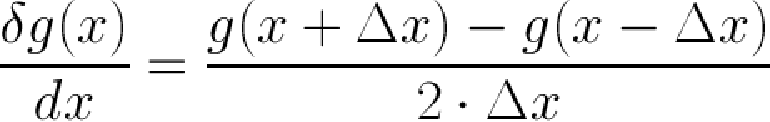
\includegraphics[width=.5\textwidth]{form1.pdf}
%\end{figure}
\begin{equation}
\frac{\delta g(x)}{dx} = \frac{g(x + \Delta x) - g(x - \Delta x)}{2 \cdot \Delta x }
\end{equation}
wobei $\Delta x = 1$. Damit hat der diskrete 1D Filter $S$ die Struktur
\begin{equation}
S = \begin{bmatrix}
1 & 0 & -1
\end{bmatrix}
\end{equation}




%\vspace{-3cm}
%\vspace{2cm}



